\section{Experimentación}

Para las diferentes mediciones necesarias para los experimentos presentados a continuación fueron realizadas sobre una CPU Intel 5200U en un sistema con 8GB de memoria RAM. Los binarios fueron compilados por \texttt{gcc 6.2.1 20160830} utilizando los flags \texttt{-O3 -std=c++11 -march=native}. El toolchain utilizado para correr las mediciones y realizar los gráficos puede encontrarse junto al código en \texttt{tools/data_analisis}.

Para las mediciones de tiempos se corre repetidamente el mismo problema no menos de 4 veces y 100ms para caso, y luego se almacena la media de las mediciones.

\subsection{Runtime de los algoritmos exactos}

\subsubsection{En función de la cantidad de nodos}

En la figura \ref{fig:time-exacto} comparamos el tiempo de ejecución del algoritmo exacto de fuerza bruta con el de backtracking.
Para ello medimos con ambos 5 casos distintos para cada combinación de cantidad de gimnasios y paradas entre 2 y 5. Además usamos siempre un tamaño de mochila mayor a tres veces la cantidad de paradas.

Como podemos observar, ambos se comportan exponencialmente pero el backtracking resulta ser cerca de un orden de magnitud mas rápido.

\begin{figure}[H]
    \centering
    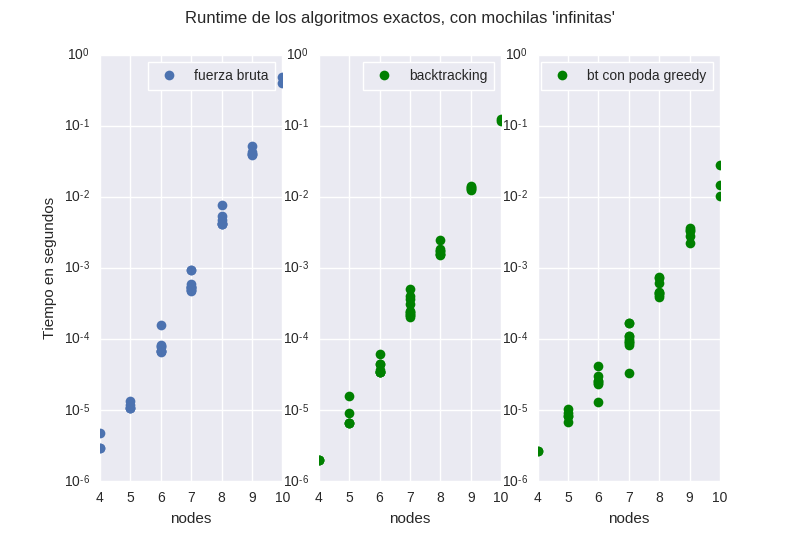
\includegraphics[width=14cm]{time-exacto}
    \caption{Tiempo de ejecución de los algoritmos exactos}
    \label{fig:time-exacto}
\end{figure}

\subsubsection{En función del tamaño de la mochila}

A continuación realizamos pruebas fijando la cantidad de gimnasios y paradas en 5 y variando el tamaño de la mochila.

Desafortunadamente vemos en la figura \ref{fig:time-exacto-moch} que dentro del intervalo de tamaños de mochila
interesantes, limitado por la cantidad de nodos que puede tener un problema a ser resuelto en un tiempo factible
(ya que si el tamaño es mayor a tres veces la cantidad de paradas, no influirá en el comportamiento del algoritmo),
no podemos determinar propiamente el comportamiento.

\begin{figure}[H]
    \centering
    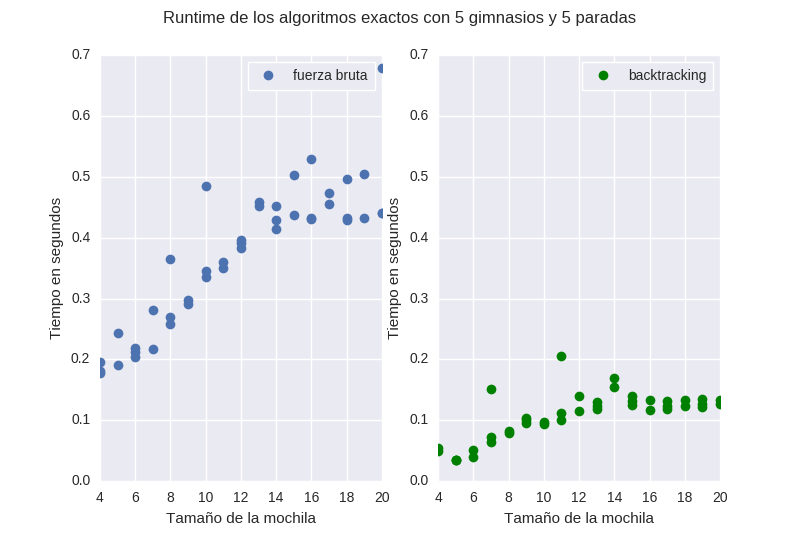
\includegraphics[width=13.5cm]{time-exacto-moch}
    \caption{Tiempo de ejecución de los algoritmos exactos al variar el tamaño de la mochila}
    \label{fig:time-exacto-moch}
\end{figure}

\subsection{Runtime de las heurísticas greedy}

\subsubsection{En función de la cantidad de nodos}

Medimos el tiempo en la figura \ref{fig:time-greedy} generando 5 casos para cada combinación de entre 1000 y 10000 gimnasios y paradas, avanzando de a 1000, y tamaño de mochila mayor a 30000.

Vemos en la figura \ref{fig:time-greedy-correlation} que estos tiempos tiempos se correlaciona fuertemente con un comportamiento cuadrático en función de la cantidad de nodos.

\begin{figure}[H]
    \centering
    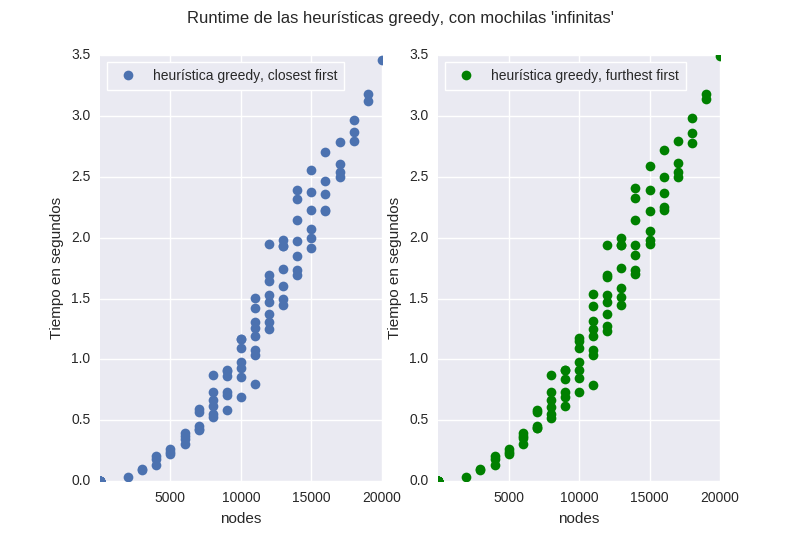
\includegraphics[width=13.5cm]{time-greedy}
    \caption{Tiempo de ejecución de las heurísticas greedy}
    \label{fig:time-greedy}
\end{figure}

\begin{figure}[H]
    \centering
    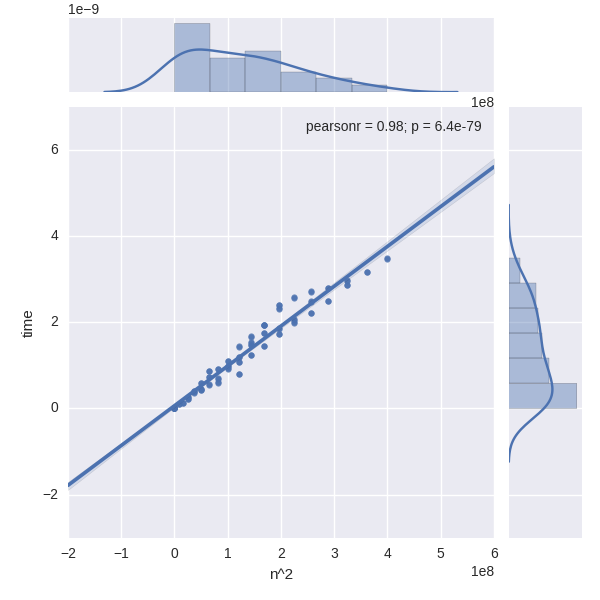
\includegraphics[width=10cm]{time-greedy-correlation}
    \caption{Correlación entre el tiempo de ejecución del greedy y una complejidad cuadrática}
    \label{fig:time-greedy-correlation}
\end{figure}

\subsubsection{En función del tamaño de la mochila}

Realizamos también pruebas fijando la cantidad de gimnasios y paradas en 2500 y variando el tamaño de la mochila entre 100 y 7500 en pasos de a 100, y nos encontramos con un comportamiento constante y con poco ruido para ambos tipos de greedy (con una correlación entre tiempo medido y tamaño de mochila de $0.170856$).

En el cuadro \ref{tab:time-greedy-moch} se encuentra una descripción de los datos medidos.

\begin{table}[H]
    \begin{center}
        \begin{tabular}{ l | r }
            count  & 76.000000 \\
            mean   &  0.215175 \\
            std    &  0.005658 \\
            min    &  0.209863 \\
            25\%   &  0.212328 \\
            50\%   &  0.213131 \\
            75\%   &  0.215283 \\
            max    &  0.239380 \\
        \end{tabular}
        \caption{Descripción de las mediciones en función del tamaño de mochila}\label{tab:time-greedy-moch}
    \end{center}
\end{table}

\subsection{Runtime de las heurísticas locales}

\subsubsection{En función de la cantidad de nodos}

Para las heurísticas locales medimos nuevamente los tiempos generando 5 casos para cada combinación de entre 10 y 100 gimnasios y paradas, avanzando de a 10, y tamaño de mochila mayor a 300. Los resultados se pueden apreciar en la figura \ref{fig:time-local}.

Podemos corroborar en la figura \ref{fig:time-local-correlation} que ambas variaciones se corresponden con un comportamiento de orden cuarto en función de la cantidad de nodos.

\begin{figure}[H]
    \centering
    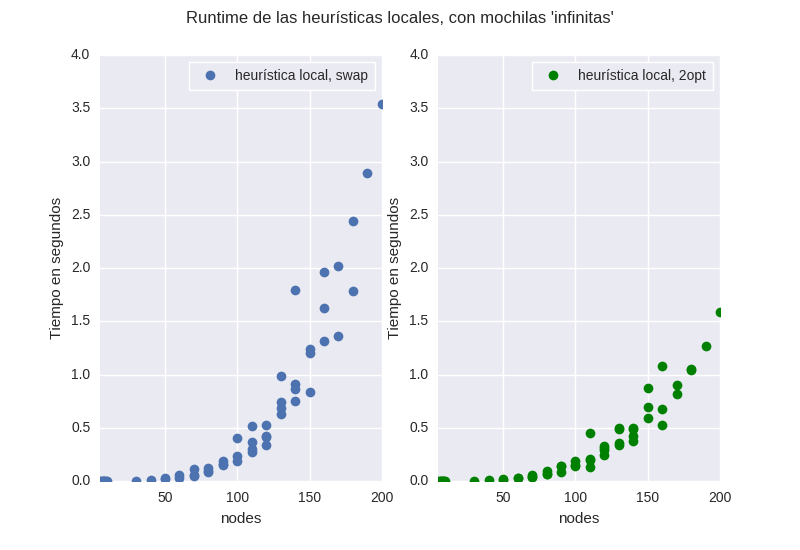
\includegraphics[width=13.5cm]{time-local}
    \caption{Tiempo de ejecución de las heurísticas locales}
    \label{fig:time-local}
\end{figure}

\begin{figure}[H]
    \centering
    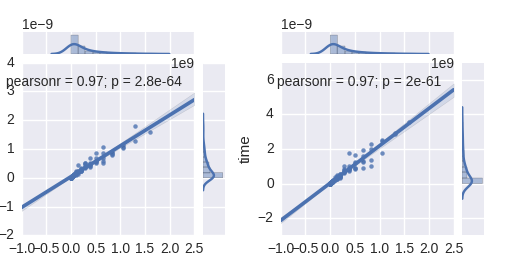
\includegraphics[width=13cm]{time-local-correlation}
    \caption{Correlación entre el tiempo de ejecución de las heurísticas locales 2opt (izquierda) y swap (derecha), con una complejidad $n^4$}
    \label{fig:time-local-correlation}
\end{figure}

\subsubsection{En función del tamaño de la mochila}

Nuevamente realizamos pruebas fijando la cantidad de gimnasios y paradas en 50 y variando el tamaño de la mochila entre 10 y 150, y nos encontramos, al igual que con el greedy, con un comportamiento constante en función de la mochila para ambas variaciones (con una correlación entre tiempo medido y tamaño de mochila de $0.259633$ para swap y de $0.265672$ para 2opt).

En el cuadro \ref{tab:time-local-moch} se encuentra una descripción de los datos medidos.

\begin{table}[H]
    \begin{center}
        \begin{tabular}{ l | r r }
            & Swap & 2opt \\
            \hline
            count  & 141.000000 & 141.000000 \\
            mean   &   0.263016 &   0.167931 \\
            std    &   0.080163 &   0.034468 \\
            min    &   0.124284 &   0.087849 \\
            25\%   &   0.214029 &   0.143264 \\
            50\%   &   0.253680 &   0.165566 \\
            75\%   &   0.297979 &   0.193758 \\
            max    &   0.566984 &   0.268200 \\
        \end{tabular}
        \caption{Descripción de las mediciones en función del tamaño de mochila}\label{tab:time-local-moch}
    \end{center}
\end{table}

\subsection{Runtime de la metaheurística GRASP}

\subsubsection{En función de la cantidad de nodos}

Para medir el comportamiento de GRASP generamos 4 instancias para cada combinación de gimnasios y mochilas entre 10 y 50, avanzando de a 5, con un tamaño de mochila superior a 150. En la figura \ref{fig:time-grasp} pueden apreciarse los resultados. Como se observa en la figura \ref{fig:time-grasp-correlation}, el comportamiento está fuertemente correlacionado a un orden 5 sobre la cantidad de nodos.

\begin{figure}[H]
    \centering
    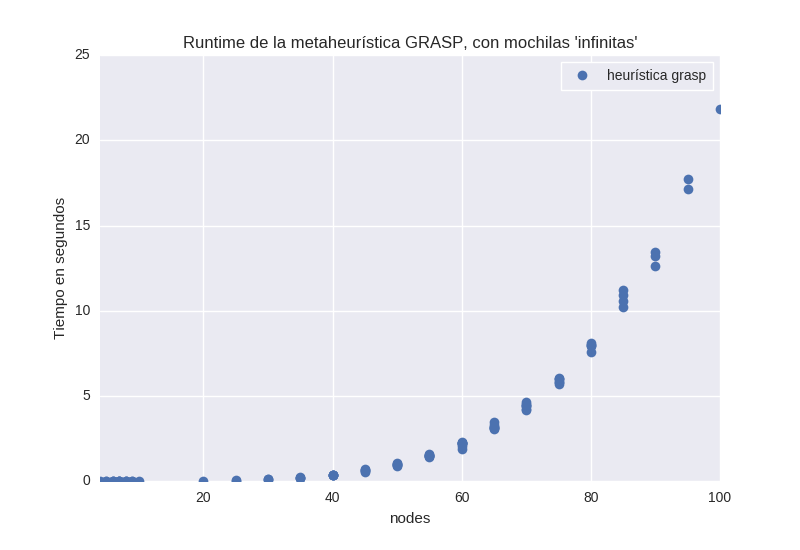
\includegraphics[width=13.5cm]{time-grasp}
    \caption{Tiempo de ejecución de la metaheurística grasp}
    \label{fig:time-grasp}
\end{figure}

\begin{figure}[H]
    \centering
    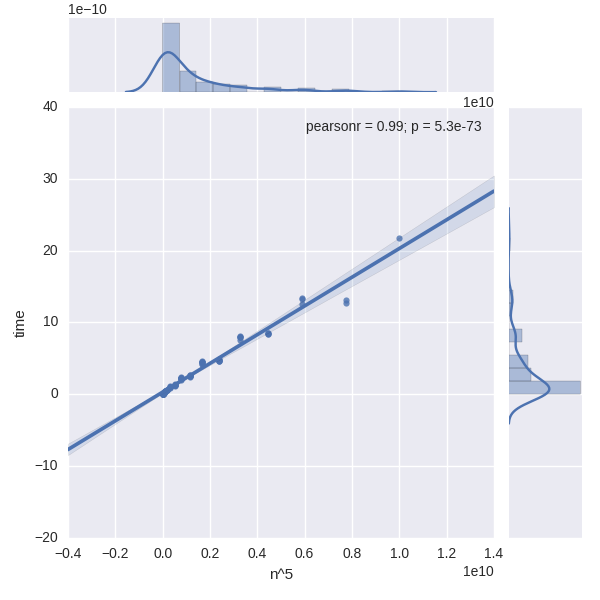
\includegraphics[width=10cm]{time-grasp-correlation}
    \caption{Correlación entre el tiempo de ejecución de grasp y una complejidad de orden 5 en función de la cantidad de nodos}
    \label{fig:time-grasp-correlation}
\end{figure}

\subsubsection{En función del tamaño de la mochila}

Para medir el tiempo de ejecución en función del tamaño de la mochila fijamos la cantidad de gimnasios y paradas en 20 y variamos la mochila entre 10 y 60. Como se aprecia en la figura \ref{fig:time-grasp-moch}, nos encontramos con que para tamaños pequeños se observa una correlación entre la mochila y el tiempo de ejecución, pero mas o menos a partir del tamaño 30 los tiempos se mantienen relativamente constantes.

Esto puede deberse a que cuando hay poco espacio el la mochila se limita la cantidad de opciones que puede tomar el algoritmo, lo que hace que termine mas temprano.

\begin{figure}[H]
    \centering
    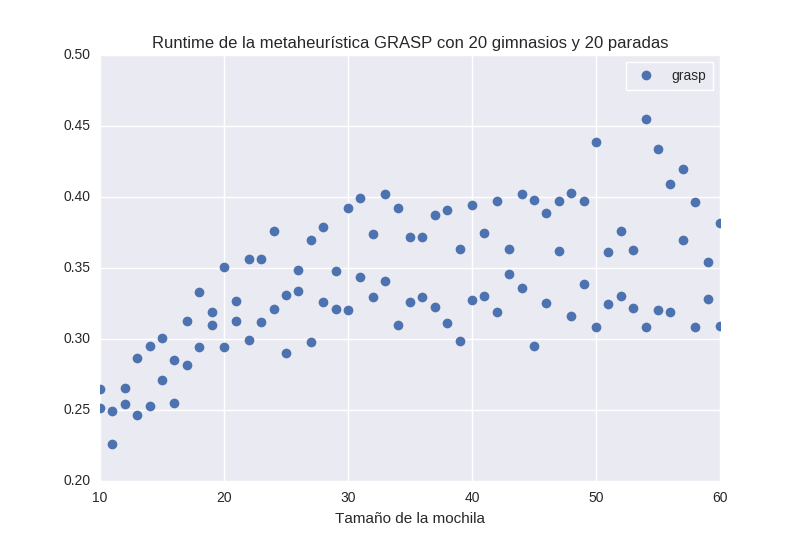
\includegraphics[width=11cm]{time-grasp-moch}
    \caption{Correlación entre el tiempo de ejecución de grasp y una complejidad de orden 5 en función de la cantidad de nodos}
    \label{fig:time-grasp-moch}
\end{figure}

\subsection{Precisión de las heurísticas}

Para medir que tan buenos son los resultados corrimos el mismo problema con cada heurística y comparamos con el resultado real,
obteniendo la proporción entre la solución encontrada y la buscada. Como el nuestro es un problema de minimización,
las proporciones siempre serán mayores o iguales a 1 (nuestras heurísticas siempre encuentran una solución posible).

Para testear problemas de mayor tamaño, tomamos como resultado de comparación el menor valor encontrado entre todas las heurísticas.

\subsubsection{Precisión en casos pequeños, comparando con el exacto}
\label{sec:precision-small}

Para cada combinación de gimnasios y paradas tal que su suma sea menor a 14 (y ambos $\geq 1$) generamos 4 casos usando el generador \texttt{random},
uno con mochila de tamaño 3, otro con tamaño igual a la cantidad de paradas, otro con el doble de las paradas
y uno con espacio igual a trues veces la cantidad de paradas.
Resolvimos estos casos con cada uno de nuestros algoritmos y comparamos las soluciones.

En la figura \ref{fig:precision-small-all} vemos las distribuciones de las precisiones para cada heurística.

Como era de esperar los algoritmos greedy suelen obtener resultados muy por encima del valor óptimo, aunque vemos que en el $75\%$
de los casos la variante closest first obtuvo un valor menor al doble del buscado.
Las heurísticas locales, especialmente la variante swap, mejoraron bastante la precision (a costa de un tiempo de ejecución bastante mas elevado).

Y por último, el GRASP obtuvo el óptimo en un $82.3\%$ de los casos.
En el cuadro \ref{tab:precision-small-grasp} se describe la distribución de su precisión.

\begin{figure}[H]
    \centering
    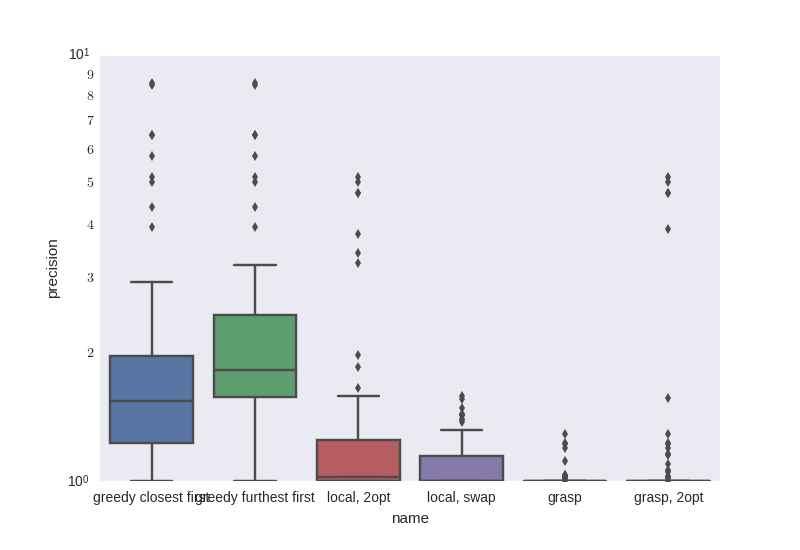
\includegraphics[width=12cm]{precision-small-all}
    \caption{Precisión comparando con el valor exacto}
    \label{fig:precision-small-all}
\end{figure}

\begin{table}[H]
    \begin{center}
        \begin{tabular}{ l | r }
            count  & 226.000000 \\
            mean   &   1.011650 \\
            std    &   0.039716 \\
            min    &   1.000000 \\
            25\%   &   1.000000 \\
            50\%   &   1.000000 \\
            75\%   &   1.000000 \\
            max    &   1.288691 \\
        \end{tabular}
        \caption{Descripción de la precisión de la metaheurística GRASP}\label{tab:precision-small-grasp}
    \end{center}
\end{table}

\subsubsection{Precisión en casos grandes, comparando con el mínimo}
\label{sec:precision-big}

A continuación generamos casos de prueba utilizando el generador \texttt{random} para todas las combinaciones de paradas y gimnasios tal que ambos
sean mayor o iguales a $10$ y su suma sea a lo sumo 40.
En cada caso variamos el tamaño de la mochila de igual forma que en la sección \ref{sec:precision-small}.

Nuevamente observamos como la variante closest first del greedy produce mejores resultados que la otra.

Además notamos que, si bien la heurística local swap no suele producir resultados muy malos,
su media es bastante peor que la variante 2opt, cuyos valores se describen en el cuadro \ref{tab:precision-big-local-2opt}.

Por último, la metaheurística grasp obtiene el mejor resultado en el $96.72\%$ de los casos.
Este número no es $100\%$ ya que existen casos donde los locales obtienen un buen resultado a partir del greedy closest first
pero el grasp, por la característica aleatoria de su ejecución, termina en una solución peor.

\begin{figure}[H]
    \centering
    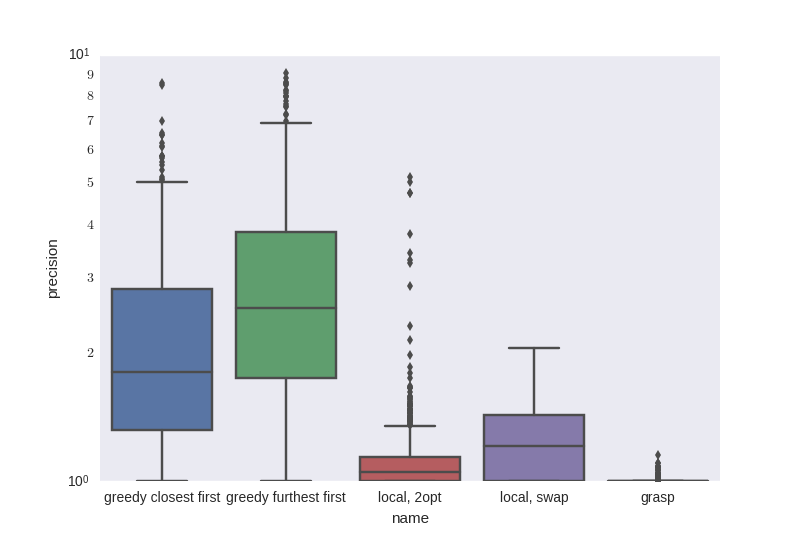
\includegraphics[width=12cm]{precision-big-all}
    \caption{Precisión comparando con el valor exacto}
    \label{fig:precision-big-all}
\end{figure}

\begin{table}[H]
    \begin{center}
        \begin{tabular}{ l | r }
            count  & 2008.000000 \\
            mean   &    1.111849 \\
            std    &    0.247017 \\
            min    &    1.000000 \\
            25\%   &    1.000000 \\
            50\%   &    1.049093 \\
            75\%   &    1.139941 \\
            max    &    5.181492 \\
        \end{tabular}
        \caption{Descripción de la precisión de la heurística local 2opt}\label{tab:precision-big-local-2opt}
    \end{center}
\end{table}

\subsubsection{Precisión en función del generador}

Utilizando las mismas variables descriptas en la sección \ref{sec:precision-big} generamos instancias con cada uno de los generadores
disponibles, para ver si la precisión variaba con los tipos de problema.

El resultado puede verse en la figura \ref{fig:precision-big-all-bygen}.
Para las instancias de \ref{zigzag} se suele conseguir buenos resultados en comparación con las \texttt{random}.
Ademas es notable que las instancias de \texttt{separated} se suelen resolver relativamente bien con las heurísticas locales y GRASP,
no así con los greedy.

\begin{figure}[H]
    \centering
    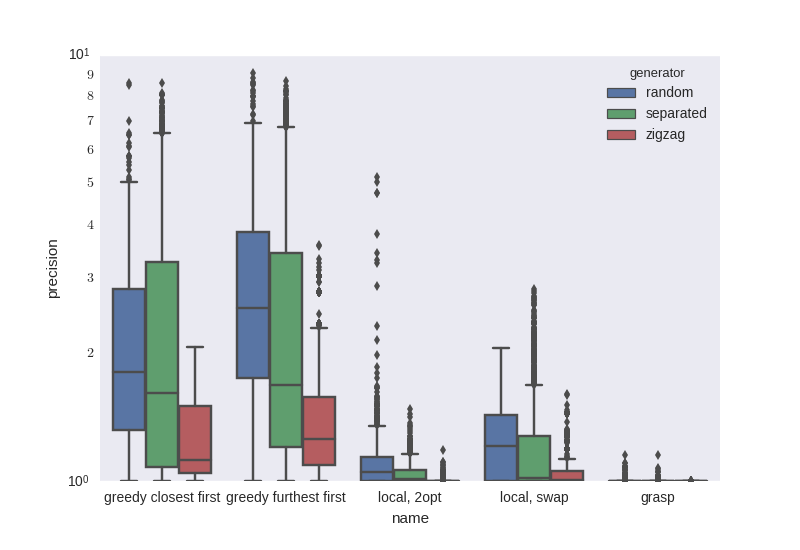
\includegraphics[width=12cm]{precision-big-all-bygen}
    \caption{Precisión comparando con el mínimo, según el generador utilizado}
    \label{fig:precision-big-all-bygen}
\end{figure}

\subsubsection{Precisión en función del tamaño de la mochila}

Quisimos también probar si el tamaño de las mochilas influía en la precisión de cada método.
Para ello tomamos los resultados obtenidos en la sección \ref{sec:precision-big} y los separamos
por el tamaño de la mochila relativo a la cantidad de paradas.

El resultado, que puede observarse en la figura \ref{fig:precision-big-all-bysize},
muestra una leve correlación para las heurísticas greedy. Las heurísticas locales y GRASP, en cambio, no parecen verse afectadas.

\begin{figure}[H]
    \centering
    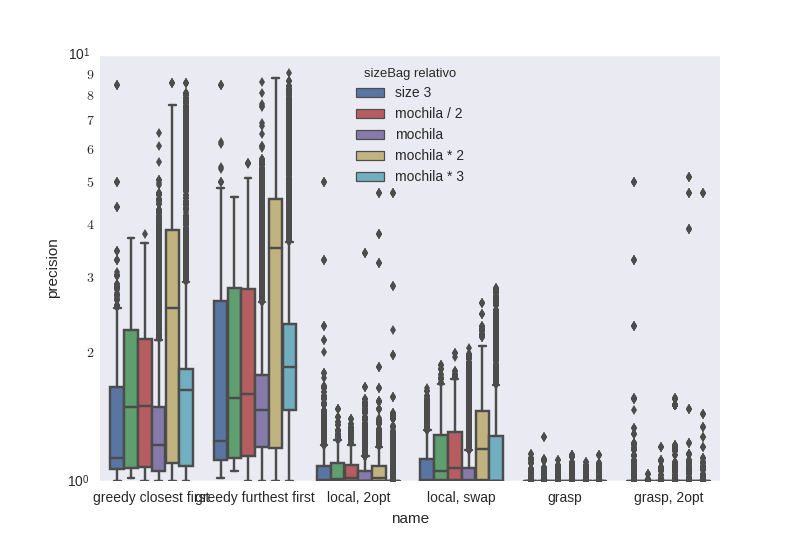
\includegraphics[width=12cm]{precision-big-all-bysize}
    \caption{Precisión comparando con el mínimo, según el tamaño relativo de la mochila}
    \label{fig:precision-big-all-bysize}
\end{figure}

